%%
%% Author: Moritz
%% 18.03.2018
%%

% Preamble
\documentclass[../../Pflichtenheft.tex]{subfiles}
\begin{document}
    \subsection{Kategorie}
    \begin{figure}[ht!]
        \begin{center}
            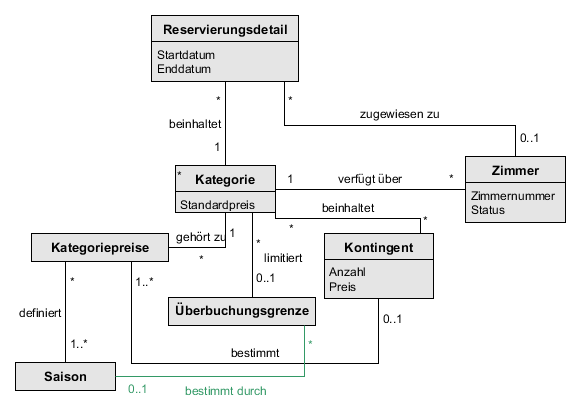
\includegraphics[width=0.5\linewidth]{assets/kategorie.png}
            \caption{Objekt 'Kategorie'} \label{kategorie_model}
        \end{center}
    \end{figure}
    Eine Kategorie verfügt über mehrere Zimmer die zu dieser Kategorie gehören.
    Außerdem gehört zu einem Kontingent eine bestimmte Anzahl an Zimmern (für den Vertragspartner: Reisebüro)
    Zu jeder Kategorie gibt es Kategoriepreise, die die Preise abhängig von mit Vertragspartnern verhandelten
    Zahlungsmodalitäten oder der Standardpreisliste festlegen, jeweils bezogen auf die Saison. Des weiteren
    ist jede Kategorie durch eine Überbuchungsgrenze beschränkt.
\end{document}